\chapter{Cryptanalysis of Block Ciphers} \label{ch:CoBC}
\label{Cryptanalysis of block ciphers}
%\input{method}
The history of cryptanalysis is long and at least as fascinating as the history of cryptography. As an example, in 1917 an article in ``Scientific American" claimed the Vigen\`{e}re cipher is ``impossible of translation" \cite{knudsen1998block}. Today, most cryptography classes at university use it as an exercise to illustrate that this claim is not true. When discussing the security of a cryptosystem, one needs to define a model works in the real world which we will use the model of Shannon \cite{shannon1949communication}.

%TO DO 插图 

The sender and the receiver share a common key $K$ over a secure channel in advance. The sender encrypts a plaintext P using the secret key $K$, sends ciphertext C over an insecure channel to the receiver. The receiver then decrypt C to P using K. The attacker has access to the insecure channel and can intercept ciphertext. In this chapter we assume that the sender and receiver use a secret key cipher $E_{K}(\cdot)$ of n-bits block size and k-bits size of key $K$. To evaluate the security we assume:

\begin{myAssumption}
	All keys are equally likely and a key K is always chosen uniformly at random
\end{myAssumption}
Also we will assume that the attacker knows all details about the cryptographic algorithm used by the sender and receiver, except the secret key. This assumption is known as Kerckhofs's Assumption \cite{kahn1996codebreakers}.
\begin{myAssumption} \label{assumption2a}
	The enemy cryptanalyst knows all details of the enciphering process and deciphering process except for the value of the secret key.
\end{myAssumption}

As an extension of the Assumption \ref{assumption2a}, we discuss the following two cases. 
\begin{myAssumption} \label{assumption2b}
	The enemy cryptanalyst knows all the details of the enciphering process and deciphering process except the value of the key and the S-Boxes (Substitution-box) which is a basic component of symmetric key algorithms which performs substitution.
\end{myAssumption}

Under this assumption, the S-Boxes are like te master key or a high level key, which is kept as security. Similar to the rotors using in German Enigma during World War II. The attacker has to first recover the S-boxes through silicon reverse engineering or try for different sets of known S-boxes, then perform normal cryptanalysis as Assumption \ref{assumption2a}.
\begin{myAssumption}
	The enemy cryptanalyst knows all the details of the enciphering process and deciphering process except that the cipher has been tweaked, for example 90\% of the cipher is what we know
\end{myAssumption}
attacker has again two steps under this assumption. First recover the cipher through reverse engineering and try different sets of known S-boxes, then perform normal cryptanalysis as Assumption \ref{assumption2a}.

\section{Classification of Attacks}
Based on these assumptions, we classify the possible attacks an attacker can do \cite{schneier1996applied}
\begin{enumerate}
	\item \textbf{Ciphertext only attack}: The attacker processes a set of intercepted ciphertexts
	\item \textbf{Known plaintext attack}: The attacker obtains $P_{1},P_{2},...,P_{s}$ a set of s plaintexts and the corresponding ciphertexts $C_{1},C_{2},...,C_{s}$
	\item \textbf{Chosen plaintext attack}: the attacker chooses a priori set of s plaintexts $P_{1},P_{2},...,P_{s}$ and obtains in some way the corresponding ciphertexts $C_{1},C_{2},...,C_{s}$
	\item \textbf{Adaptively chosen plaintext attack}: The attacker chooses a set of plaintext $P_{1},P_{2},...,P_{s}$ interactively as he obtains the corresponding ciphertext $C_{1},C_{2},...,C_{s}$. That is the attacker chooses $P_{1}$, obtains $C_{1}$, \textbf{then} chooses $P_{2}$ etc.
	\item \textbf{Chosen ciphertext attacks}: For symmetric ciphers these are similar to those of chosen plaintext attack and adaptively chosen plaintext attack
\end{enumerate}

The chosen text attacks are the most powerful attacks. However, they are also unrealistic in many applications. If there exist redundancy in plaintext space, it will be very hard for an attacker to find an encrypted non-meaningful plaintexts send by the sender, and similarly hard to get ciphertexts decrypted. But if a system is secure against an adaptively chosen text attack then it is also secure against all other attacks.

Modern cryptanalysis on block ciphers has been very focused on finding the secret key $K$. However, there are other serious attacks for public key cryptography which do not find the secret key. \cite{knudsen1994block} classified the types of breaks in his paper as follows:
\begin{enumerate}
	\item \textbf{Total break}: An attacker finds the secret key $K$
	\item \textbf{Global deduction}: An attacker finds an algorithm $A$, functionally equivalent to $E_{K}(\cdot)(or\ D_{K}(\cdot))$ without knowing the key $K$.
	\item \textbf{Instance (local) deduction}: An attacker finds the plaintext (ciphertext) of an intercepted ciphertext (plaintext), which he did not obtain from the legitimate sender
	\item \textbf{Information deduction}: An attacker gains some information about the key, plaintexts or ciphertexts, which he did not get directly from sender and which he did not have before the attack.
\end{enumerate} 
This classification is hierarchical, i.e., if a total break is possible, then a global deduction is possible etc.

\paragraph{Data Requirement} Attacks can also be characterised by resources they require. Those resources include time complexity, memory usage and data requirements. The first two types of resources are very obvious, however it is worth to point out data requirement is also a key component that makes an attack can work in practices. Full plaintext and ciphertext pairs are not easy to obtain in real world. Some of attacks works only if all possible plaintext and ciphertext pairs for a single key is known, and some of the attacks can work with multiple key scenarios. 
\section{Brute-force Attack}
Brute-force attack or exhaustive key search is the most general attack that can be applied to any block cipher. All block ciphers are totally breakable in a ciphertext only attack, just simply by trying all the possible keys one by one and checking whether the computed plaintext is meaningful. This attack requires the computation of about $2^{k}$ encryptions. The dimension of the key space $k$, which is the length of the key, determines the practical feasibility of performing a brute-force attack. For modern block ciphers, brute force is always possible in theory but computationally infeasible in practise.
\section{Linear Cryptanalysis}
Linear cryptanalysis is a known plaintext attack on block ciphers. It was popularised by Matsui in 1993 \cite{matsui1994linear}. A preliminary version of the attack on FEAL was described in 1992 \cite{matsui1993new}. Although the published attack on DES requires $2^{43}$ known plaintexts which is not very practical, it still was a great improvement in experimental cryptanalysis. 

Linear cryptanalysis is based on finding affine approximations to the action of a cipher which hold with high probability. The attacker exploits linear approximations of some bits of the plaintext, ciphertext and key. In the attack on the DES (or on DES-like iterated ciphers) the linear approximations are obtained by combining approximations for each round under the assumption of independent round keys. 

The attacker hopes to find an expression (equation \ref{eq:test}), which holds with probability $p_{L} \neq \frac{1}{2}$ over all keys \cite{matsui1994linear}, such that $\epsilon = \mid p_{L} - \frac{1}{2} \mid$, call the bias, is maximal. 
\begin{equation} \label{eq:test}
(P\cdot\alpha)\oplus(C\cdot\beta)=(K\cdot\gamma)
\end{equation}
where $P,C,\alpha,\beta,\gamma$ are m-bit strings and where `$\cdot$' denotes the dot product.

Given an approximation (equation \ref{eq:test}) a linear attack using $N$ plaintexts and the $N$ corresponding ciphertexts goes as follows\cite{matsui1994linear}. 

\begin{enumerate}
	
	\item for all plaintexts, $P$, and ciphertexts, $C$, let $T$ be the number of times the left hand side of equation \ref{eq:test} is 0.
	\item if $T > \frac{N}{2}$ guess that $K \cdot \gamma = 0$, otherwise guess that $K \cdot \gamma = 1$ (majority vote).
	
\end{enumerate}
By using the above method, the attacker can find one bit of information about the secret key, $K \cdot \gamma$. However, the above linear attack is not very efficient, as it only finds one bit of information about the key. In \cite{matsui1994linear}, Matsui also showed an extended linear attack which finds more key bits. Instead of approximating the first and last round, the extended linear attack simply repeat the attack for all values of the relevant key bits in those two rounds by using the following approximation equation (equation \ref{eq:linear2}). 
\begin{equation} \label{eq:linear2}
(P \cdot \alpha) \oplus (C \cdot \beta) \oplus (F(P_{R},K_{1}) \cdot \alpha_{1}) \oplus (F(C_{R},K_{r}) \cdot \alpha_{r}) = (K \cdot \gamma)
\end{equation}
where $P_{R}, C_{R}$ are the right halves of the plaintexts and ciphertexts. $K_{1}$ and $K_{R}$ are the key bits affecting the linear approximation in the first and $r$th rounds. We refer reader to \cite{matsui1994linear} for more details.


Kaliski and Robshaw showed an improved linear attack using multipe linear approximations in \cite{kaliski1994linear}. In \cite{kilian1996protect} Knudsen and Robshaw introduced a linear attack using non-linear approximations in the outer rounds of an block cipher. Both of these are not been able to show an significant improvement compared to Matsui's linear attack. The attacks seem best suited for ciphers with large S-boxes, such as LOKI \cite{brown1990loki} \cite{kilian1996protect}. In 2004, new attacks were introduced to attack Feistel schemes in \cite{courtois2004feistel} which have a small improvements than Matsui's work.

\section{Differential Cryptanalysis}
Differential cryptanalysis is based on tracking changes in the differences between two messages as theypass through the consecutive rounds of encryption. It is one of the oldest classical attacks on modern block ciphers. In cryptographic literature, it was first described and analysed by Biham and Shamir and applied to DES algorithm in the early 1990s \cite{biham1993differential}. However, Coppersmith, a member of the IBM team which designed DES \cite{coppersmith1994data,coppersmith2000development,courtois2003s}, has reported that this attack was already known to IBM designers around 1974. It was known under the name of T-attack or Tickle attack, and DES had already been designed to resist this type of attack. A detailed discussion of specific original design criteria of DES can be found in \cite{courtois2003s}. Moreover, it appers that IBM had agreed with the NSA that the design criteria of DES should not be made public, precisely because it would ``weaken the competitive advantage the United States enjoyed over other countries in the field of cryptography" cf. \cite{coppersmith1994data,coppersmith2000development} 

Today, differential cryptanalysis is extremely well known. Numerous authors studied various aspects of differential cryptanalysis extensively in the 1990s. Apart from DES, differential cryptanalysis has also been successfully applied to a wide range of iterated ciphers \cite{knudsen1993cryptanalysis,massey1994safer}.  Recent research work also showed a great success using differential cryptanalysis to break Russian standard GOST  \cite{gostdc0,gostdc1} and NSA lightweight cipher SIMON and SPECK \cite{biryukov2014differential,alkhzaimi2013cryptanalysis}

The data requirements for differential cryptanalysis works with multiple key scenario, where linear cryptanalysis requires data on single key. This is the main reason why differential cryptanalysis is considered more stronger than linear cryptanalysis \cite{courtois2005best}.

The main task of Differential cryptanalysis is to study the propagation of input differences from round to round inside the encryption system, and find specific differences which propagate with high probability. Such pairs of input-output can be used to recover some bits of the secret key. In general, differential cryptanalysis exposes the non-uniform distribution of the output differences given one or several input differences.

\begin{mydef} \label{df_difference}
	a \textbf{difference} between two bit strings, $X$ and $X^{'}$ of equal length as $$\triangle X = X \otimes (X^{'})^{-1}$$
	where $\otimes$ is the group operation on the group of bit strings used to combine the key with the text input in the round function and where $(X)^{-1}$ is the inverse element of X with respect to $\otimes$
\end{mydef}

Generally, the selection of the operator $\otimes$ depends on the way the round subkeys are introduced in each round. As in many ciphers use XOR for the key application in round function, the operator in definition \ref{df_difference} usually is exclusive-or ($\oplus$).

The attacker then computes the differences of the corresponding ciphertexts, hoping to detect statistical patterns in their distribution. The resulting pair of differences is called a differential. Their statistical properties depend upon the internal structure of the cipher. The attacker aim to find one particular ciphertext difference which is especially frequent. In this way, the cipher can be distinguished from random.

\paragraph{Truncated Differentials} \mbox{ } \\
Truncated Differential Cryptanalysis is a generalization of differential cryptanalysis developed by Lars Knudsen \cite{Knudsen95}. Unlike differential cryptanalysis which studies the propagation of the full difference between two plaintexts, truncated differential cryptanalysis consider differences that are partially determined, as in some ciphers, it is possible and advantageous to predict the values of parts of the differences after each round. This technique have been successfully applied to many block ciphers such as Russian standard GOST \cite{gostdc2,TheoPhD,courtois2015can}. Truncated differential is defined as follow: \cite{Knudsen95}.

\begin{mydef}
	A differential that predicts only parts of an n-bit value is called a truncated differential. More formally, let(a,b) be an $i$-round differential. If $a^{'}$ is a subsequence of a and $b^{'}$, then ($a^{'},b^{'}$) is called an $i$-round truncated differential.
\end{mydef}

A truncated differential can be considered as a collection of differentials. For example, let ($a^{'},b$) be the truncated differential of an  n-bit block cipher, where $a^{'}$ specifies the least $n^{'} < n$ significant bits of the plaintext difference and b specifies the ciphertext difference of length n. This differential is a collection of all $2^{n-n^{'}}$ differentials (a,b), where a is any value that truncated to the $n^{'}$ least significant bits is $a^{'}$. 

\section{Algebraic Attacks} \label{sec:AA}
%What is AA?

In general the security of a given block cipher will grow exponentially with the number of rounds and so does the number of required plaintext-ciphertext pairs which are needed in a linear and differential cryptanalytic attack. However, in most cases, only a few plaintext-ciphertext pairs are available for cryptanalysis, linear or differential attacks are not expected to succeed. Thus, a new method needs to be invented which will be able to recover the secret key with only a few information is available.

Claude Shannon, has once suggested that the security of a cipher should be related to the difficulty of solving the underlying system of equations and deriving the key: 


\begin{quotation}
	\textit{``if we could show that solving a certain system requires at least as much work as solving a system of simultaneous equations in a large number of unknowns, of a complex type, then we would have a lower bound of sorts for the work characteristic"} \cite{Shannon}. 
\end{quotation}
This is the core concept behind algebraic attacks. 

An algebraic attack is a form of known plaintext attack which consists of the following two steps:

%How AA works?
\begin{enumerate}
	\item \textbf{Modelling}: Describe the cipher as a multivariate system of polynomial equations over a small finite field (like GF(2) ) or logical constraints in terms of the secret key K, the plaintext P and the ciphertext C. $$ {f_{1}(K,P,C)=0,...f_{r}(K,P,C)=0 \Longleftrightarrow E(K,P) = C}$$
	
	\item \textbf{Solving}: Solve the underlying multivariate system of equations and obtain the secret key. In order to reduce the complexity of solving the system we substitute to the system all known plaintext/ciphertext pairs. The more the pairs the more
	the equations we obtain involving the key bits. For many known attack this can make the problem easier to solve.
\end{enumerate}

Generally, each module of a block cipher can be described with a set of algebraic equations. Put these algebraic equation together, we can get a large precise system describing the whole cipher. The main idea of algebraic attack is to establish a series of low complexity algebraic equations of initial plaintext and ciphertext, and then find the secret key by solving the equations. Such equation systems are normally very large systems of quadratic multivariate polynomial equations over GF(2). Each variable of such equation system represents a state-bit of the encryption algorithm. Then the variables which representing state-bits from the initial round are set according to values of the plaintext, and similarly variables which representing state-bits from the last round are set according to values to the ciphertext. Therefore, the security of a block cipher depends on whether there exist an efficient algorithm to solve such large and sparse multivariate polynomial equations. If we can solve the equation system faster than exhaustive key search attack, the cipher will be broken (in academic sense).

In addition, some high profile cryptanalysis problems in public key cryptography can be written in such a form which contains a ``block cipher topology" \footnote{which is how we / Dr. Courtois classify the equations proposed by Semaev in 2015 \cite{courtois2002cryptanalysis,CourtoisBlockEnigmaSlides,cryptoeprint:2015:310}}. Such equations have similar structure as a block cipher, where the beginning inputs and final outputs variables are easy to get and the middle part of the equation system are very hard to analyse (see figure \ref{fig:blockciphertopology}). One example is Semaev's summation polynomial equations for elliptic curve \cite{semaev2004summation,cryptoeprint:2015:310} see section \ref{sec:SemaevCipher}.      

\begin{figure}[h!]
	\centering
	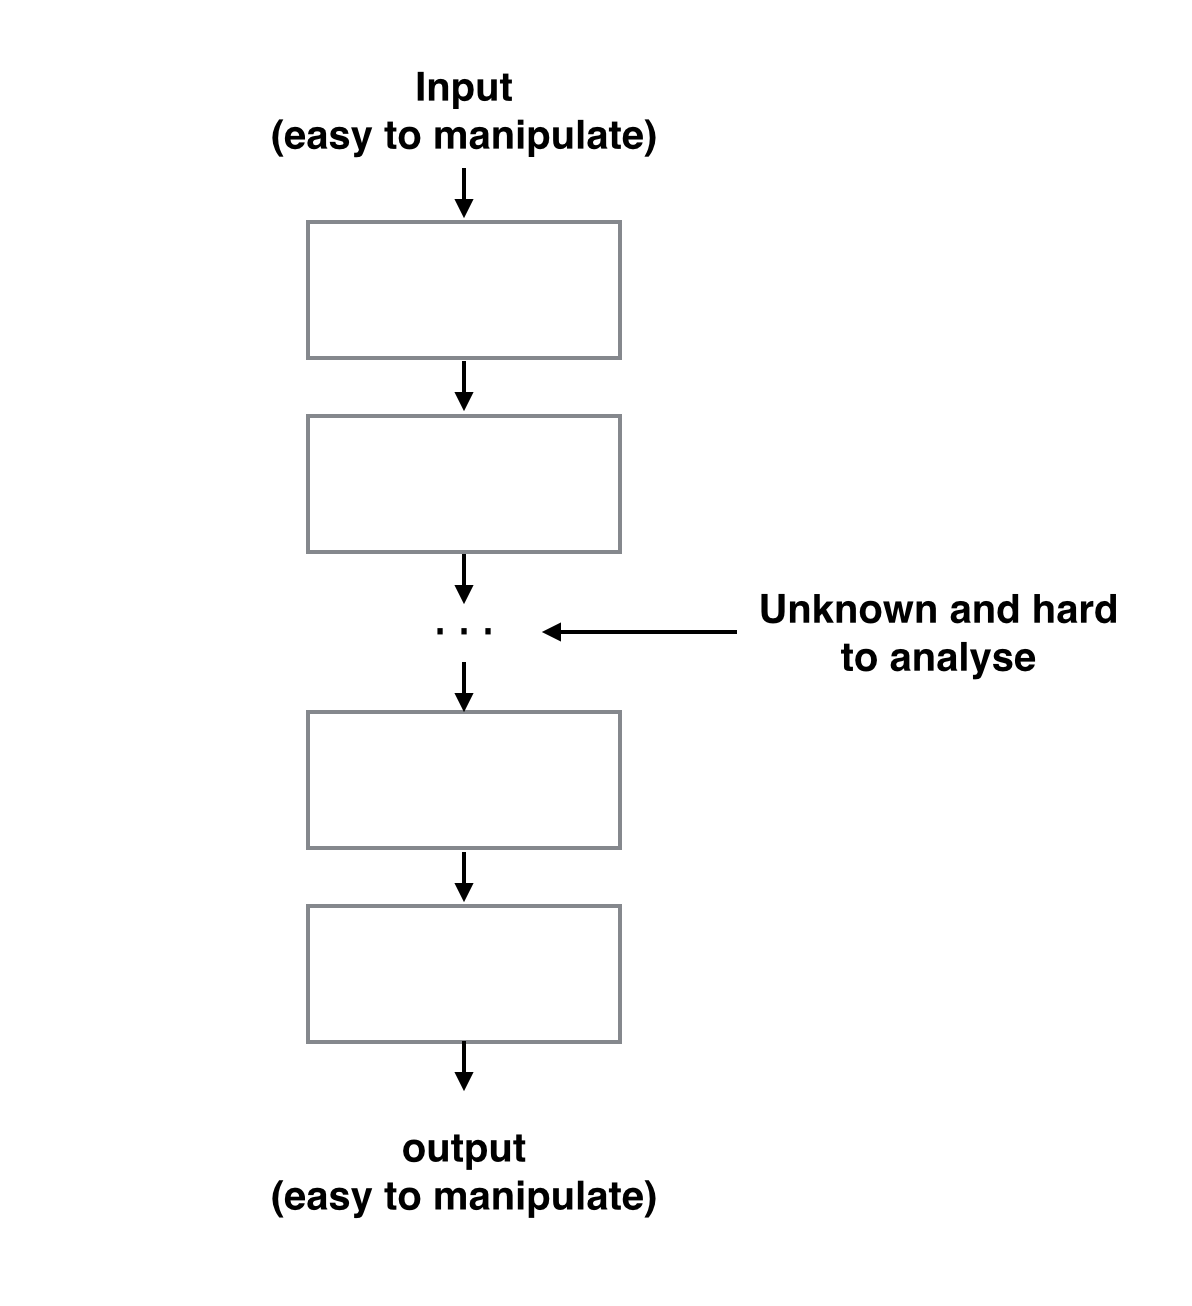
\includegraphics[width=130mm]{./pics/block_cipher_topology2.png}	
	\caption{Block cipher topology: attackers are easy to control or manipulate the inputs and outputs but very hard to analyse variables in the middle}
	\label{fig:blockciphertopology}
\end{figure}	



\subsection{Algebraic Attacks Solving Stage}
Solving a random system of multivariate non-linear boolean equations is an NP-hard problem \cite{fraenkel1980complexity}. As many cryptographic primitives can be described by a sparse multivariate non-linear system of equations over $GF(2)$ or any other algebraic systems. Several techniques were develop in order to tackle the problem of solving such equations. A classic approach is to use techniques from algebraic geometry and especially Gr\"{o}bner bases algorithms to solve the system of equations \cite{faugere1999new}. But most of the times they do not lead to solutions in practise due to the extremely high memory requirements. Then, some heuristic techniques were developed called \textit{linearisation} \cite{courtois2000efficient}, where all the non-linear terms are replaced by an independent linear variable and the resulting linear system can be solved using Gaussian elimination \cite{sepehrdad2012statistical}. However, it requires that there are enough linearly independent equations and the initial system is highly over-defined and sparse. Then, XL algorithm \cite{courtois2000efficient,courtois2002cryptanalysis} was developed to make the system over-defined, by addition of new equations to the current system. The proposal of XL made it possible to solve the multi-order nonlinear equations within polynomial time, which accelerated the development of the algebraic attacks. Then researchers focus mainly on the fast solutions to the algebraic equation systems. 

In the past few years, researchers try to solve the problem by using tools and software, such as SAT solvers. Nicolas Courtois is the pioneer of bringing SAT solvers into action in the area of symmetric cryptanalysis. His paper \cite{cryptoeprint:2007:024,BardCourtoiJeffersonConv} described how to covert such equations to a format which can be solved automatically by SAT solvers. The advantage of such technique is that SAT solvers can perform reasonably well and do not require a lot of memory as in case of Gr$\ddot{o}$bner basis-based techniques \cite{grobner}. The only disadvantage is the unpredictability of its complexity. The first algebraic attack on reduce round block cipher DES was done by Courtois and Bard in  \cite{DEScourtois}. Later in 2008, first algebraic attack on full block cipher KeeLoq \cite{courtois2008algebraicKeeLoq}. In the past 10 years, SAT solvers were used for attacks on block ciphers such as GOST\cite{courtois2012contradiction,gostac} and Chinese block cipher SMS4 \cite{erickson2010algebraic},  stream ciphers such as Crypto-1, HiTag2 and Bivium \cite{soos2009extending,courtois2009practical}, and also MiFare Classic smart cards \cite{courtois2008algebraic}.

Another method, is to use ElimLin algorithm \cite{ElimLinR}. ElimLin stands for \textbf{Elim}inate \textbf{Lin}ear and it is a simple algorithm for solving polynomial systems of multivariate equations over small finite fields and was initially proposed as a single tool by Courtois to attack DES and CTC/CTC2 ciphers \cite{DEScourtois}. It is also known as ``inter-reduction'' step in all major algebra systems.

Its main aim is to reveal some hidden linear equations existing in the ideal generated by the system of
polynomials. ElimLin is composed of two sequential stages, as follows:

\begin{itemize}
	\item \textbf{Gaussian Elimination:} Discover all the linear equations in the linear span of initial equations.
	\item \textbf{Substitution:} Variables are iteratively eliminated in the whole system based on linear equations found until there is no linear equation left.
\end{itemize}

Given an initial multivariate system of equations over $S^0$ in $\mathbb{F}_2[x_1,x_2,..,x_n]$, then the ElimLin is formally described as below.

\begin{algorithm}
	\caption{ElimLin Algorithm}
	\begin{algorithmic}
		\STATE \textbf{Input:} $S^0=\{f_1,f_2,...,f_m\} \in \mathbb{F}_2[x_1,x_2,..,x_n]$
		\STATE \textbf{Output:} An updated system of equations $S^T$ and a system of linear equations $S_L$
		\STATE 1. Set $S_L\leftarrow{\O}$ and $S^T \leftarrow S^0$ and $k\leftarrow 1$
		\STATE 2. \textbf{Repeat}
		\STATE For some ordering of equations and monomials perform $Gauss(S^T)$ to eliminate non-linear monomials
		\STATE Set $S_{L'} \leftarrow$ Linear Equations from $Gauss(S^T)$
		\STATE Set $S^T\leftarrow Gauss(S^T)\backslash S_{L'}$
		\STATE Let $l \in S_{L'}$, $l$ non-trivial (if unsolvable then \emph{terminate})
		\STATE Let $x_{i_k}$ a monomial in $l$
		\STATE Substitute $x_{i_k}$ in $S^T$ and $S_{L'}$ using $l$
		\STATE Insert $l$ in $S_L$
		\STATE $k\leftarrow k+1$
	\end{algorithmic}
\end{algorithm}

This method is iterated until no linear equation is obtained in the linear
span of the system. Intuitively, ElimLin seems to work better in cases where there is low
non-linearity since this implies the existence of more linear equations.
MC is another notion of non-linearity \cite{FourMNL,OptimiPaper2}
and possibly such method
may work sufficiently well in cryptographic primitives of low MC.


